% Report source. Figures are report/figures/*.pdf and tables are report/generated/tab_*.tex (both regenerated by
% `code/make_figures.py` and `code/make_tables.py`); every result number in the text is a macro from generated/numbers.tex.
% `% macros:` lines list macro-name prefixes (a trailing * means "all macros starting with"); code/check_reproduction.py
% checks that every macro in numbers.tex is listed in exactly one section.
\documentclass[10pt,a4paper,twocolumn]{article}

%%%%%%%%%%%%%%%%%%%%%%%%%%%%%%%%%%%% PREAMBLE (course template, two-column) %%%%%%%%%%%%%%%%%%%%%%%%%%%%%%%%%%%%
\usepackage[numbers,sort]{natbib}
\usepackage{amsfonts,amsmath,amssymb}
\usepackage{graphicx,booktabs}
\usepackage{libertine}
\usepackage[a4paper,margin=1.8cm,columnsep=0.7cm]{geometry}
\usepackage{hyperref}
\hypersetup{
    colorlinks = true,
    linkcolor = blue,
    urlcolor  = blue,
    citecolor = blue,
    anchorcolor = blue}
\urlstyle{same}
\graphicspath{{figures/}}
% Generated by code/make_figures.py from results/ ; do not edit.
\newcommand{\numHfourspearmanellipsoid}{0.97}
\newcommand{\numHfourspearmanrosenbrock}{0.97}
\newcommand{\numHoneKfourDfive}{-1.50 [-1.70, -0.93]}
\newcommand{\numHoneKfourDten}{-0.86 [-0.99, -0.74]}
\newcommand{\numHoneKfourDtwo}{-1.75 [-2.12, -1.38]}
\newcommand{\numHoneSellipsoid}{0.34 [-0.55, 1.14]}
\newcommand{\numHoneSkfour}{0.90 [0.44, 1.35]}
\newcommand{\numHoneSrosenbrock}{0.65 [0.03, 1.22]}
\newcommand{\numHoneellipsoidDeight}{-2.37 [-2.59, -2.04]}
\newcommand{\numHoneellipsoidDfive}{-2.98 [-3.15, -2.61]}
\newcommand{\numHoneellipsoidDten}{-2.01 [-2.21, -1.88]}
\newcommand{\numHoneellipsoidDthree}{-2.89 [-3.42, -2.61]}
\newcommand{\numHoneellipsoidDtwo}{-2.35 [-3.12, -1.50]}
\newcommand{\numHonefinalellipsoideight}{-0.66 [-1.28, -0.36]}
\newcommand{\numHonefinalellipsoidfive}{-0.24 [-1.13, 0.31]}
\newcommand{\numHonefinalellipsoidten}{-0.13 [-0.51, 0.10]}
\newcommand{\numHonefinalellipsoidthree}{-0.72 [-1.30, 0.01]}
\newcommand{\numHonefinalellipsoidtwo}{0.94 [0.44, 1.52]}
\newcommand{\numHonefinalrosenbrockeight}{0.56 [0.26, 0.83]}
\newcommand{\numHonefinalrosenbrockfive}{0.03 [-0.19, 0.23]}
\newcommand{\numHonefinalrosenbrockten}{0.72 [0.58, 0.84]}
\newcommand{\numHonefinalrosenbrockthree}{-0.76 [-0.92, -0.31]}
\newcommand{\numHonefinalrosenbrocktwo}{-1.06 [-1.44, 0.07]}
\newcommand{\numHonerosenbrockDeight}{-0.66 [-1.02, -0.53]}
\newcommand{\numHonerosenbrockDfive}{-0.98 [-1.25, -0.76]}
\newcommand{\numHonerosenbrockDten}{-0.82 [-1.12, -0.49]}
\newcommand{\numHonerosenbrockDthree}{-1.50 [-1.72, -0.86]}
\newcommand{\numHonerosenbrockDtwo}{-1.48 [-1.96, -1.07]}
\newcommand{\numablationalignedcubic}{1.82}
\newcommand{\numablationaligneddefault}{0.87}
\newcommand{\numablationalignediso}{2.42}
\newcommand{\numablationcontrastcubicdefault}{-0.96 [-1.08, -0.68]}
\newcommand{\numablationdrotcubic}{0.60 [0.49, 0.69]}
\newcommand{\numablationdrotdefault}{1.56 [1.27, 1.63]}
\newcommand{\numablationdrotiso}{0.01 [-0.09, 0.15]}
\newcommand{\numablationfloorcubic}{-0.08 [-0.24, 0.11]}
\newcommand{\numablationfloordefault}{0.00 [-0.09, 0.25]}
\newcommand{\numablationflooriso}{0.01 [-0.11, 0.14]}
\newcommand{\numablationrotatedcubic}{2.39}
\newcommand{\numablationrotateddefault}{2.29}
\newcommand{\numablationrotatediso}{2.45}
\newcommand{\numalphaall}{1.82 [1.80, 1.84]}
\newcommand{\numalphadgeten}{2.02 [1.99, 2.06]}
\newcommand{\numcstardefinedellipsoideight}{19}
\newcommand{\numcstardefinedellipsoidfive}{19}
\newcommand{\numcstardefinedellipsoidten}{17}
\newcommand{\numcstardefinedellipsoidthree}{19}
\newcommand{\numcstardefinedellipsoidtwo}{16}
\newcommand{\numcstardefinedrosenbrockeight}{7}
\newcommand{\numcstardefinedrosenbrockfive}{15}
\newcommand{\numcstardefinedrosenbrockten}{1}
\newcommand{\numcstardefinedrosenbrockthree}{19}
\newcommand{\numcstardefinedrosenbrocktwo}{19}
\newcommand{\numcstarellipsoideight}{5.77 [IQR 2.68, 11.25]}
\newcommand{\numcstarellipsoidfive}{1.39 [IQR 0.52, 3.56]}
\newcommand{\numcstarellipsoidten}{59.85 [IQR 28.85, 103.71]}
\newcommand{\numcstarellipsoidthree}{0.80 [IQR 0.58, 1.38]}
\newcommand{\numcstarellipsoidtwo}{0.99 [IQR 0.60, 3.05]}
\newcommand{\numcstarrosenbrockeight}{7.81 [IQR 3.81, 19.01]}
\newcommand{\numcstarrosenbrockfive}{3.39 [IQR 1.20, 8.87]}
\newcommand{\numcstarrosenbrockten}{48.54 [IQR 48.54, 48.54]}
\newcommand{\numcstarrosenbrockthree}{0.33 [IQR 0.15, 0.63]}
\newcommand{\numcstarrosenbrocktwo}{0.48 [IQR 0.30, 0.93]}
\newcommand{\numdrotboardreplicate}{-0.05 [-0.12, 0.15]}
\newcommand{\numdrotboardrotated}{0.85 [0.71, 0.98]}
\newcommand{\numdrotboisoreplicate}{0.10 [-0.04, 0.29]}
\newcommand{\numdrotboisorotated}{-0.09 [-0.25, 0.18]}
\newcommand{\numdrotcmareplicate}{-0.04 [-0.27, 0.21]}
\newcommand{\numdrotcmarotated}{0.16 [0.00, 0.41]}
\newcommand{\numdrotsepcmareplicate}{-0.07 [-0.24, 0.15]}
\newcommand{\numdrotsepcmarotated}{0.87 [0.72, 1.07]}
\newcommand{\numdrotsobolreplicate}{0.05 [-0.11, 0.13]}
\newcommand{\numdrotsobolrotated}{-0.01 [-0.16, 0.10]}
\newcommand{\numdrotturboreplicate}{0.00 [-0.09, 0.25]}
\newcommand{\numdrotturborotated}{1.56 [1.27, 1.63]}
\newcommand{\numeprobtwohundrednarrowcma}{0.00}
\newcommand{\numeprobtwohundrednarrowipop}{0.00}
\newcommand{\numeprobtwohundrednarrowlogei}{0.00}
\newcommand{\numeprobtwohundrednarrowsobol}{0.07}
\newcommand{\numeprobtwohundrednarrowucb}{0.00}
\newcommand{\numeprobtwohundredwidecma}{0.80}
\newcommand{\numeprobtwohundredwideipop}{0.80}
\newcommand{\numeprobtwohundredwidelogei}{0.80}
\newcommand{\numeprobtwohundredwidesobol}{1.00}
\newcommand{\numeprobtwohundredwideucb}{0.67}
\newcommand{\numeprobtwothousandnarrowcma}{0.00}
\newcommand{\numeprobtwothousandnarrowipop}{0.10}
\newcommand{\numeprobtwothousandnarrowsobol}{0.87}
\newcommand{\numeprobtwothousandwidecma}{0.80}
\newcommand{\numeprobtwothousandwideipop}{1.00}
\newcommand{\numeprobtwothousandwidesobol}{1.00}
\newcommand{\numethreeipoppooled}{0.32 [0.25, 0.39]}
\newcommand{\numethreeucbminuslogeinarrow}{0.00 [0.00, 0.00]}
\newcommand{\numethreeucbminuslogeiwide}{-0.13 [-0.27, -0.03]}
\newcommand{\numgapmedboardaligned}{0.95}
\newcommand{\numgapmedboardrotated}{1.75}
\newcommand{\numgapmedboisoaligned}{1.60}
\newcommand{\numgapmedboisorotated}{1.60}
\newcommand{\numgapmedcmaaligned}{2.73}
\newcommand{\numgapmedcmarotated}{2.97}
\newcommand{\numgapmedsepcmaaligned}{2.08}
\newcommand{\numgapmedsepcmarotated}{3.04}
\newcommand{\numgapmedsobolaligned}{3.76}
\newcommand{\numgapmedsobolrotated}{3.72}
\newcommand{\numgapmedturboaligned}{0.87}
\newcommand{\numgapmedturborotated}{2.29}
\newcommand{\numinteractionBO}{0.89 [0.54, 1.20]}
\newcommand{\numinteractionCMA}{0.76 [0.62, 0.93]}
\newcommand{\numoverheadboardellipsoideight}{4.10}
\newcommand{\numoverheadboardellipsoidfive}{1.87}
\newcommand{\numoverheadboardellipsoidten}{10.65}
\newcommand{\numoverheadboardellipsoidthree}{1.10}
\newcommand{\numoverheadboardellipsoidtwo}{0.79}
\newcommand{\numoverheadboardrosenbrockeight}{2.53}
\newcommand{\numoverheadboardrosenbrockfive}{1.08}
\newcommand{\numoverheadboardrosenbrockten}{6.94}
\newcommand{\numoverheadboardrosenbrockthree}{0.76}
\newcommand{\numoverheadboardrosenbrocktwo}{0.69}
\newcommand{\numrankcorrntwohundredaligned}{1.00}
\newcommand{\numrankcorrntwohundredrotated}{0.44}
\newcommand{\numrhontwohundredaligned}{1.00}
\newcommand{\numrhontwohundredrotated}{0.17}


\newcommand{\Drot}{\Delta_{\mathrm{rot}}}
\renewcommand{\dbltopfraction}{0.9}\renewcommand{\topfraction}{0.9}\renewcommand{\textfraction}{0.07}
\renewcommand{\dblfloatpagefraction}{0.8}\renewcommand{\floatpagefraction}{0.8}\setcounter{dbltopnumber}{4}
%%%%%%%%%%%%%%%%%%%%%%%%%%%%%%%%%%%%%%%%%%%%%%%%%%%%%%%%%%%%%%%%%%%%%%%%%%%%%%%%%%%%%%%%%%%%%%%%%%%%%%%%%%%%%%%%%

\begin{document}

\title{When Does Bayesian Optimisation Beat CMA-ES? Rotation, Dimension and Evaluation Cost}
\author{}
\date{\today}
\maketitle

{\bf Group Composition:}
\begin{enumerate}
\item Melisa Abigail Thevandi, A0288030J, e1300520@u.nus.edu
\end{enumerate}

{\bf Github Repository:} \url{https://github.com/melisathevandi/bo-vs-cmaes}

\section{Introduction and hypotheses}
% sources: predictions.md (H1--H5 and the follow-up)
% figures: none
% tables: none
% macros: none
Gaussian-process Bayesian optimisation (BO) and CMA-ES are two standard methods for expensive black-box minimisation
\citep{frazier2018tutorial,hansen2016tutorial}. A comparison of high-dimensional BO methods
with vanilla BO and CMA-ES on the 24 BBOB functions found BO better than CMA-ES for limited evaluation budgets, with trust
regions as the most promising improvement of BO \citep{santoni2024hdbo}; standard BO also works much better in high
dimensions than previously thought when the lengthscale prior is scaled with the dimension \citep{hvarfner2024vanilla}.
This study asks which problem properties decide the winner at a given budget (axis alignment, dimension relative to
budget, multimodality and evaluation cost), and whether BO's advantage reflects problem--method fit rather than general
superiority.

The hypotheses were committed before the main runs (\texttt{predictions.md}).
\textbf{H1}: BO's lead over CMA-ES at a fixed number of evaluations per dimension shrinks as the dimension grows.
\textbf{H2}: axis-aligned methods (ARD-kernel BO, separable CMA-ES) gain on aligned problems and lose that gain under
rotation; isotropic BO and full CMA-ES are approximately rotation invariant.
\textbf{H3}: the chance of finding a narrow global basin falls with its width; restarts (IPOP) help CMA-ES at larger
budgets; UCB beats LogEI on the narrowest basins.
\textbf{H4}: the break-even evaluation cost $c^*$, above which BO is faster in wall-clock time, rises with the budget.
\textbf{H5}: the evaluations CMA-ES needs to learn the geometry scale as $d^\alpha$ with $\alpha$ below 2 at finite $d$,
as derived from its learning rates. A follow-up on TuRBO's rotation penalty was registered after the first results and
before its own runs.

Later changes are dated amendments or addenda committed before the affected numbers were computed. H1 names
$\kappa=10^4$, but the E1 configurations use $\kappa=100$; an amendment records that H1 was tested at $\kappa=100$ and
that its $d=20$ part was not run, and a $\kappa=10^4$ supplement was added after the E1 analysis. Before any E2 result was
read, the rule ``stop if the aligned-replicate CI excludes 0'' was replaced by a 99\% interval with a tolerance, and the
follow-up gained noise-floor runs before its runs.

\section{Methods and experimental design}
% sources: configs/*.toml, code/methods/*.py, code/problems.py, analysis_addendum_*.md
% figures: none
% tables: tab:design (inline table of experiments, from configs/)
% macros: none
\paragraph{Problems.}
All problems are defined on $[0,1]^d$. The ellipsoid is $f(x)=\sum_i \kappa^{(i-1)/(d-1)} y_i^2$ with $y=R(x-x^*)$,
aligned ($R=I$) or rotated by a random orthogonal $R$ with the same optimum; an independent \emph{aligned replicate} gives
the noise floor of a rotation effect. The other functions are
a shifted Rosenbrock function, a quadratic in $d=20$ that depends on only $d_{\mathrm{eff}}=2$ directions, and a
two-dimensional decoy-basin function $f=\min(B,D)$ with a broad basin $B\geq1$ and a narrow global basin of width $w$, so
that $f<1$ exactly within $w$ of the narrow optimum.

\paragraph{Methods.}
BO uses a BoTorch Gaussian process with a Mat\'ern-5/2 kernel, ARD or isotropic, the dimension-scaled lengthscale prior
of Hvarfner et al.~\citep{hvarfner2024vanilla} and LogEI, which reformulates expected improvement to avoid numerically
vanishing values and gradients \citep{ament2023logei} (UCB with $\beta=4$ in E3). Hyperparameters are refitted from
defaults at every iteration up to $n=100$ and every ten iterations afterwards (checked in the Appendix). TuRBO-1 uses local models in a
trust region scaled by the ARD lengthscales, because global-model BO is often not competitive on difficult
high-dimensional problems \citep{eriksson2019turbo}; its settings are the reference defaults. CMA-ES (pycma) starts from a
uniform random point with $\sigma_0=0.3$ of the box width, default population and pycma's bound handling; sep-CMA-ES
restricts the covariance to a diagonal, which gives linear complexity but is not rotation invariant \citep{ros2008sepcma};
IPOP restarts with a doubled population. Sobol sampling is the model-free reference (Table~\ref{tab:design}).

\begin{table*}[t]\centering\footnotesize\setlength{\tabcolsep}{3pt}
\begin{tabular}{@{}p{0.11\textwidth}p{0.25\textwidth}p{0.09\textwidth}p{0.12\textwidth}p{0.07\textwidth}p{0.29\textwidth}@{}}
\toprule
Experiment & Problems & $d$ & Budget (evaluations) & Seeds & Methods \\
\midrule
E2 primary & ellipsoid $\kappa=10^4$: aligned, rotated, aligned replicate & 10 & 500 & 0--29 & ARD-BO, iso-BO, TuRBO, CMA-ES, sep-CMA-ES, Sobol \\
E2 secondary & as E2 primary & 10 & 500; 10{,}000 & 0--29 & CMA-ES with $\sigma_0=0.15$; CMA-ES long runs \\
E2 low dimension & quadratic, $d_{\mathrm{eff}}=2$: aligned, rotated & 20 & 500 & 0--19 & ARD-BO, iso-BO, TuRBO, CMA-ES, Sobol \\
E1 & rotated ellipsoid $\kappa=100$; shifted Rosenbrock & 2, 3, 5, 8, 10 & 200, 200, 400, 640, 1000 & 0--19 & ARD-BO, CMA-ES, Sobol \\
E1 long runs & as E1 & 2, 3, 5, 8, 10 & up to 50{,}000 & 0--19 & CMA-ES (until pycma terminates) \\
E1 supplement & rotated ellipsoid $\kappa=10^4$ & 2, 5 & 200, 400 & 0--19 & ARD-BO, CMA-ES, Sobol \\
H5 & rotated ellipsoid $\kappa=10^4$, no bounds, no termination & 2 to 80 (11 values) & up to $100\,d^2$ & 20 per $d$ & CMA-ES \\
E3 & decoy basin, $w\in\{0.2,0.1,0.05,0.025,0.0125\}$ & 2 & 200; 2000 & 0--29 & LogEI-BO, UCB-BO, CMA-ES, IPOP, Sobol; at 2000 only CMA-ES, IPOP, Sobol \\
Follow-up & as E2 primary & 10 & 500 & 0--29 & TuRBO: ARD kernel with cubic region; isotropic kernel \\
Sensitivity & rotated ellipsoid $\kappa=100$; Rosenbrock & 10; 5 & 500; 400 & 1000--1009 & 6 CMA-ES and 6 BO configurations \\
\bottomrule
\end{tabular}
\caption{Experiments as run (from \texttt{configs/*.toml}). All runs use the unit box (except H5), CPU only and one
thread per worker. A seed fixes the problem instance and the method's random stream, so all methods in an experiment see
the same instances; seeds from 1000 are held out from the main runs. BO and TuRBO budgets include $2d$ initial Sobol
points.}
\label{tab:design}
\end{table*}

\paragraph{Fair comparison.}
All methods see the same instances for a seed, and all comparisons are paired by seed. BO and TuRBO start from $2d$
Sobol points that count against the budget; CMA-ES starts from one random point. Tuning effort is equal: six configurations per method (CMA-ES: $\sigma_0\times$ population; BO: initial design $\times$
Mat\'ern smoothness) on held-out seeds of two pilot problems, with a rule fixed in advance to keep the default unless an
alternative is better on both problems with a paired CI excluding 0. No alternative met the rule, so all defaults were
kept. The recommendation is the best evaluated point.

\paragraph{Metric, cost and statistics.}
Performance is the $\log_{10}$ gap $f(\text{best so far})-f^*$ on the true objective, floored at $10^{-12}$, with budgets
counted in function evaluations as in standard benchmarking \citep{hansen2021coco}. Method overhead is the wall-clock time
of a run minus the time inside the objective, i.e.\ model fitting and acquisition. If BO reaches a target gap after
$n_{BO}$ evaluations and CMA-ES after $n_{CMA}>n_{BO}$, with cumulative overheads $T_{BO}$ and $T_{CMA}$, the break-even
cost per evaluation is $c^*=(T_{BO}-T_{CMA})/(n_{CMA}-n_{BO})$: BO is faster in total time when an evaluation costs more.
Comparisons report the median paired difference with a 95\% percentile bootstrap CI over seeds (10{,}000 resamples);
differences between dimensions resample both seed sets independently; success rates use Wilson intervals. The rotation
penalty is $\Drot=\log_{10}\text{gap(rotated)}-\log_{10}\text{gap(aligned)}$, paired by seed, and its noise floor is the
same difference between the aligned replicate and the aligned instance.

\section{Rotation and axis alignment (E2, H2)}
% figures: fig1_e2_primary (E2 primary: final gap and rotation penalty), fig2_e2_lowdim (convergence, relevance ratio, rank correlation)
% tables: tab_e2, tab_lowdim
% macros: gapmed*, drot*, interaction*, rhon*, rankcorrn*
\begin{figure*}[t]\centering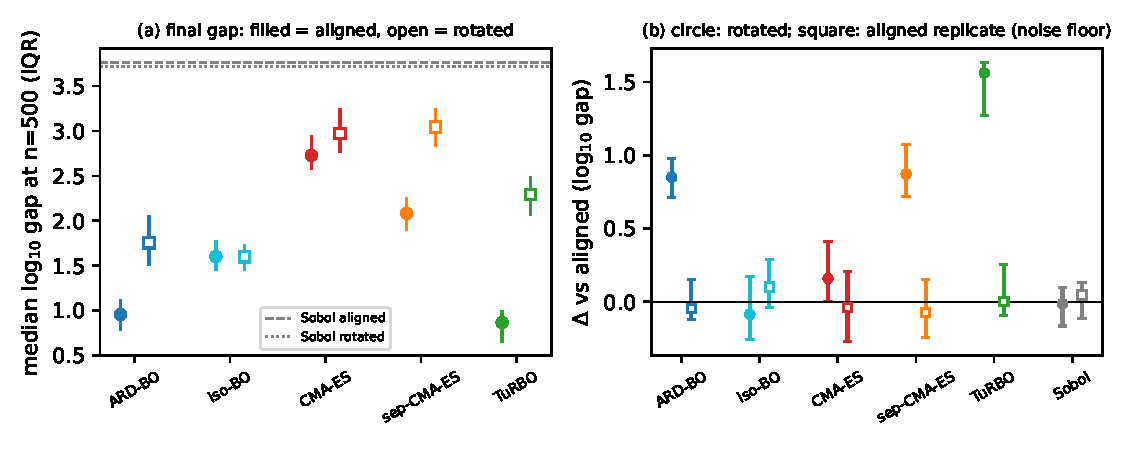
\includegraphics[width=\linewidth]{fig1_e2_primary}\caption{E2 primary: ellipsoid,
$\kappa=10^4$, $d=10$, 500 evaluations, 30 seeds. (a) Median final $\log_{10}$ gap with IQR, aligned (filled) and rotated
(open); horizontal lines: Sobol. (b) Paired rotation penalty $\Drot$ (circles) and aligned-replicate noise floor
(squares), median with 95\% bootstrap CI; positive means worse after rotation.}\label{fig:e2}\end{figure*}
\begin{figure*}[t]\centering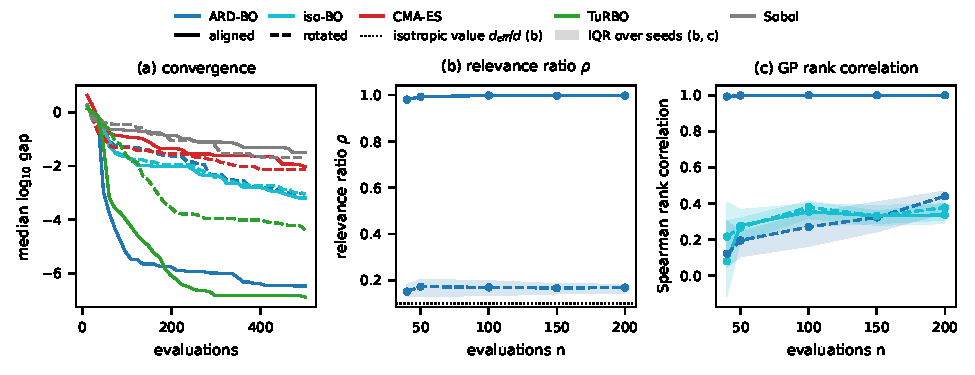
\includegraphics[width=\linewidth]{fig2_e2_lowdim}\caption{E2 low effective dimension:
quadratic in $d=20$ with two relevant directions, aligned (solid) or rotated (dashed), 20 seeds. (a) Median $\log_{10}$
gap. (b) Relevance ratio $\rho$ of the fitted ARD kernel (share of kernel sensitivity in the relevant directions;
dotted: isotropic value $d_{\mathrm{eff}}/d$). (c) Spearman correlation between GP posterior mean and true function
near the incumbent. Bands: IQR over seeds.}\label{fig:lowdim}\end{figure*}
\begin{table*}[t]\centering\resizebox{\textwidth}{!}{\begin{tabular}{lcc}
\toprule
Method & $\Delta_{rot}$ [95\% CI] & Noise floor [99\% CI] \\
\midrule
ARD-BO & 0.85 [0.71, 0.98] & -0.05 [-0.14, 0.24] \\
iso-BO & -0.09 [-0.25, 0.18] & 0.10 [-0.08, 0.35] \\
TuRBO & 1.56 [1.27, 1.63] & 0.00 [-0.19, 0.39] \\
CMA-ES & 0.16 [0.00, 0.41] & -0.04 [-0.31, 0.26] \\
sep-CMA-ES & 0.87 [0.72, 1.07] & -0.07 [-0.28, 0.23] \\
Sobol & -0.01 [-0.16, 0.10] & 0.05 [-0.12, 0.15] \\
Interaction: ARD-BO $-$ iso-BO & 0.89 [0.54, 1.20] &  \\
Interaction: sep-CMA-ES $-$ CMA-ES & 0.76 [0.62, 0.93] &  \\
\bottomrule
\end{tabular}
}\caption{E2 primary ($d=10$,
$\kappa=10^4$, 500 evaluations, 30 paired seeds). $\Drot$: median paired difference in $\log_{10}$ gap, rotated minus
aligned (95\% bootstrap CI). Noise floor: aligned replicate minus aligned (99\% CI, pre-registered check). Interactions:
difference of the two methods' $\Drot$; H2 requires both positive with CIs excluding 0.}\label{tab:e2}\end{table*}
\begin{table*}[t]\centering\resizebox{\textwidth}{!}{\begin{tabular}{lccccc}
\toprule
Instance & $\rho$ median [IQR] & Threshold & Runs meeting & Rank corr. ARD-BO & Rank corr. iso-BO \\
\midrule
aligned & 0.998 [0.997, 0.999] & $\rho$ $\geq$ 0.5 & 20/20 & 1.00 [1.00, 1.00] & 0.34 [0.31, 0.40] \\
rotated & 0.168 [0.143, 0.182] & $\rho$ $\leq$ 0.2 & 17/20 & 0.44 [0.35, 0.47] & 0.38 [0.29, 0.40] \\
\bottomrule
\end{tabular}
}\caption{E2 low effective dimension at
$n=200$ ($d=20$, $d_{\mathrm{eff}}=2$, 20 runs per instance): ARD-BO relevance ratio $\rho$ with the pre-registered
threshold and the runs meeting it, and Spearman rank correlation of the GP posterior mean with the true function, median
[IQR]. The isotropic value of $\rho$ is $d_{\mathrm{eff}}/d$.}\label{tab:lowdim}\end{table*}

\paragraph{Question and setup.}
Does the ARD kernel exploit axis alignment and lose it under rotation, as sep-CMA-ES does? The primary endpoint was fixed
in advance (Table~\ref{tab:design}); a $d=20$ problem with two relevant directions shows what the kernel learns.

\paragraph{Result.}
Both pre-registered interactions are positive with CIs excluding 0 (Table~\ref{tab:e2}, Figure~\ref{fig:e2}b): ARD-BO minus
isotropic BO $\numinteractionBO$ and sep-CMA-ES minus CMA-ES $\numinteractionCMA$ decades. Rotation costs ARD-BO
$\Drot=\numdrotboardrotated$, sep-CMA-ES $\numdrotsepcmarotated$ and TuRBO $\numdrotturborotated$; isotropic BO
($\numdrotboisorotated$) and Sobol ($\numdrotsobolrotated$) are unaffected, and full CMA-ES has a small penalty
($\numdrotcmarotated$). No noise floor was flagged. Rotation shrinks BO's lead without reversing the ranking
(Figure~\ref{fig:e2}a): the median final $\log_{10}$ gap of ARD-BO rises from $\numgapmedboardaligned$ to
$\numgapmedboardrotated$ and that of TuRBO from $\numgapmedturboaligned$ to $\numgapmedturborotated$, while CMA-ES is at
$\numgapmedcmaaligned$ and $\numgapmedcmarotated$, isotropic BO at $\numgapmedboisoaligned$ on both instances and Sobol at
$\numgapmedsobolaligned$. On the low-effective-dimension problem (Figure~\ref{fig:lowdim}, Table~\ref{tab:lowdim}) the
relevance ratio of ARD-BO at $n=200$ is $\numrhontwohundredaligned$ when aligned and $\numrhontwohundredrotated$ when
rotated, close to the isotropic value, and the GP ranks candidates almost perfectly when aligned (rank correlation
$\numrankcorrntwohundredaligned$) but not when rotated ($\numrankcorrntwohundredrotated$). Both thresholds on $\rho$ hold.

\paragraph{Interpretation.}
H2 is supported. The ARD kernel is a diagonal metric that cannot represent an off-axis subspace, so its aligned advantage
is one of fit, not of method.
% CHECK: comparison of medians only; no paired test of BO against CMA-ES on the rotated instance was pre-registered.
At this budget every BO variant nevertheless stays ahead of both CMA-ES variants after rotation.

\paragraph{Caveat.}
All E2 runs are bounded. A rotation audit of CMA-ES (E0, Appendix) found its invariance intact without bounds but not with
them, so the CMA-ES part of H2 was informed by E0 rather than tested independently.
% CHECK: qualitative statement from results/summary/e2_cma_long_reach.csv (no macro).
CMA-ES is far from converged at 500 evaluations: long runs reach BO's final gap only after several times that budget.

\section{Dimension, budget and cost (E1, H1, H4, H5)}
% figures: fig3_e1_h5 (regime map, H1 statistic at both kappa, CMA-ES learning time)
% tables: tab_cstar, tab_h5
% macros: Hone*, Hfour*, cstar*, overhead*, alpha*
\begin{figure*}[t]\centering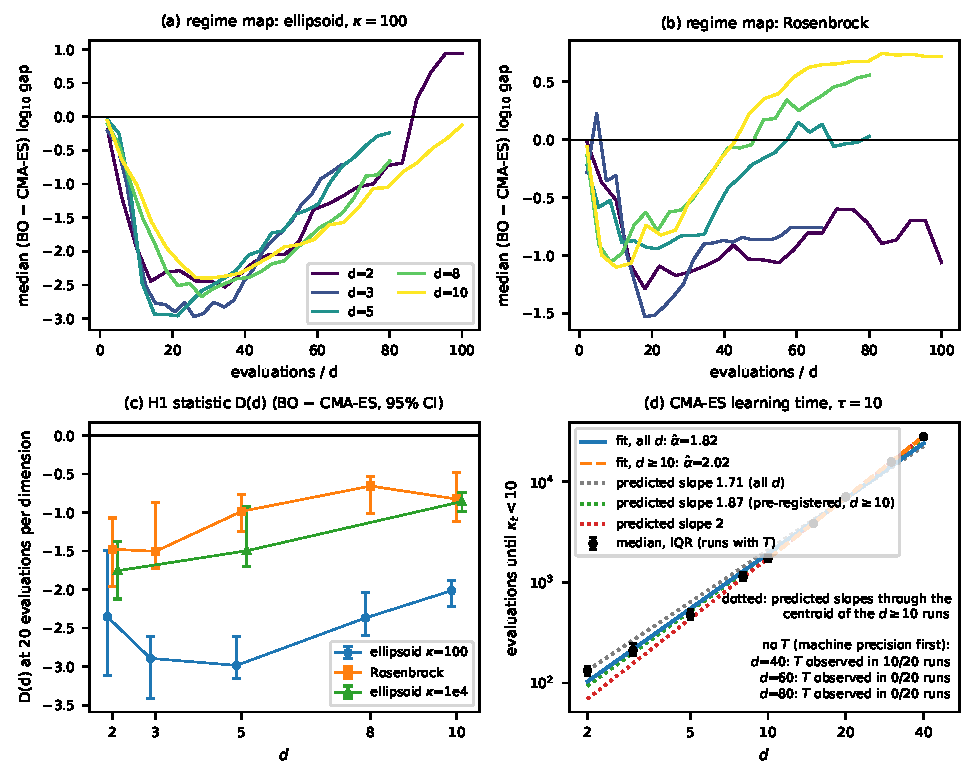
\includegraphics[width=\linewidth]{fig3_e1_h5}\caption{E1 and H5. (a, b) Median paired
difference in $\log_{10}$ gap, BO minus CMA-ES (negative: BO better), against evaluations per dimension, one line per $d$,
for the rotated ellipsoid with $\kappa=100$ (a) and Rosenbrock (b); 20 seeds. (c) H1 statistic $D(d)$, the same
difference at 20 evaluations per dimension (95\% bootstrap CI), for both E1 problems and the $\kappa=10^4$ supplement.
(d) CMA-ES learning time $T$ (evaluations until the condition number of $C^{1/2}HC^{1/2}$ falls below 10): median and IQR,
least-squares fits over all $d$ and $d\geq10$, and predicted slopes 1.71 (through the all-$d$ centroid), 1.87 and 2
(through the $d\geq10$ centroid).}\label{fig:e1}\end{figure*}
\begin{table*}[t]\centering\resizebox{\textwidth}{!}{\begin{tabular}{rcccc}
\toprule
$d$ & Ellipsoid $c^*$ (s) median [IQR] & Seeds & Rosenbrock $c^*$ (s) median [IQR] & Seeds \\
\midrule
2 & 0.99 [0.60, 3.05] & 16/20 & 0.48 [0.30, 0.93] & 19/20 \\
3 & 0.80 [0.58, 1.38] & 19/20 & 0.33 [0.15, 0.63] & 19/20 \\
5 & 1.39 [0.52, 3.56] & 19/20 & 3.39 [1.20, 8.87] & 15/20 \\
8 & 5.77 [2.68, 11.25] & 19/20 & 7.81 [3.81, 19.01] & 7/20 \\
10 & 59.85 [28.85, 103.71] & 17/20 & 48.54 [48.54, 48.54] & 1/20 \\
\bottomrule
\end{tabular}
}\caption{Break-even cost $c^*$ (seconds
per evaluation) of ARD-BO against CMA-ES on the E1 problems, at each BO run's own final gap (budgets 200, 200, 400, 640,
1000 for $d=2,3,5,8,10$): median and IQR over the seeds where CMA-ES needs more evaluations than BO, using the CMA-ES long
runs. BO is faster in total time when an evaluation costs more than $c^*$.}\label{tab:cstar}\end{table*}
\begin{table*}[t]\centering\resizebox{\textwidth}{!}{\begin{tabular}{clcccc}
\toprule
$\tau$ & Fit & $\hat\alpha$ [95\% CI] & Runs & Contains 1.87 & Contains 2 \\
\midrule
10 & all d & 1.818 [1.798, 1.839] & 170 & no & no \\
10 & d $\geq$ 10 & 2.022 [1.988, 2.056] & 90 & no & yes \\
3 & all d & 1.743 [1.705, 1.782] & 100 & no & no \\
3 & d $\geq$ 10 & 1.718 [1.574, 1.854] & 22 & no & no \\
100 & all d & 1.942 [1.923, 1.960] & 218 & no & no \\
100 & d $\geq$ 10 & 2.174 [2.155, 2.192] & 138 & no & no \\
\bottomrule
\end{tabular}
}\caption{H5: fitted exponent $\hat\alpha$ of
CMA-ES learning time against dimension (least squares on $\log T$ against $\log d$, 95\% bootstrap CI over seeds within
each $d$) for thresholds $\tau$ on the condition number. Primary endpoint: $\tau=10$, $d\geq10$, predicted 1.87. Runs
without a measured $T$ are excluded.}\label{tab:h5}\end{table*}

\paragraph{Question and setup.}
How does BO's lead depend on dimension and budget, when does its overhead pay off, and how fast does CMA-ES learn the
geometry? E1 compares ARD-BO, CMA-ES and Sobol for $d=2$ to 10 (Table~\ref{tab:design}). The H1 statistic, fixed before the analysis, is $D(d)$, the median paired difference
BO minus CMA-ES at 20 evaluations per dimension, and $S=D(10)-D(2)$: $S\geq0.5$ supports the registered size, $S\leq0$
refutes H1, and values in between support the direction only. H5 uses separate unbounded CMA-ES runs.

\paragraph{Result (H1).}
BO is ahead at 20 evaluations per dimension at every $d$ (Figure~\ref{fig:e1}c). On the ellipsoid
$D(d)=\numHoneellipsoidDtwo$, $\numHoneellipsoidDthree$, $\numHoneellipsoidDfive$, $\numHoneellipsoidDeight$ and
$\numHoneellipsoidDten$ for $d=2,3,5,8,10$, so $S=\numHoneSellipsoid$: direction only, with a CI containing 0. On Rosenbrock
$D(2)=\numHonerosenbrockDtwo$ and $D(10)=\numHonerosenbrockDten$, so $S=\numHoneSrosenbrock$, meeting the registered size.
The $\kappa=10^4$ supplement gives $D=\numHoneKfourDtwo$, $\numHoneKfourDfive$ and $\numHoneKfourDten$ at $d=2,5,10$ and
$S=\numHoneSkfour$. In the regime maps (Figure~\ref{fig:e1}a, b) CMA-ES closes the gap later in the run. At the final budget CMA-ES is ahead on Rosenbrock from $d=8$
($\numHonefinalrosenbrockeight$ at $d=8$, $\numHonefinalrosenbrockten$ at $d=10$); on the ellipsoid the two are level at
$d=10$ ($\numHonefinalellipsoidten$) and CMA-ES is ahead at $d=2$ ($\numHonefinalellipsoidtwo$).

\paragraph{Result (H4).}
BO's overhead on the ellipsoid grows from $\numoverheadboardellipsoidtwo$\,s per evaluation at $d=2$ to
$\numoverheadboardellipsoidten$\,s at $d=10$ (Rosenbrock: $\numoverheadboardrosenbrocktwo$\,s and
$\numoverheadboardrosenbrockten$\,s), against well under a millisecond for CMA-ES. The median $c^*$ on the ellipsoid rises
from \numcstarellipsoidtwo\,s at $d=2$ to \numcstarellipsoidten\,s at $d=10$ (Table~\ref{tab:cstar}), with a Spearman
correlation with the budget of $\numHfourspearmanellipsoid$ (Rosenbrock $\numHfourspearmanrosenbrock$): H4 is supported. On
Rosenbrock at $d=10$, $c^*$ exists for only $\numcstardefinedrosenbrockten$ of 20 seeds, because CMA-ES usually reaches
BO's final gap with fewer evaluations; there is then no cost at which BO is faster.

\paragraph{Result (H5).}
The fitted exponent is $\hat\alpha=\numalphadgeten$ for $d\geq10$ and $\numalphaall$ over all $d$ (Figure~\ref{fig:e1}d,
Table~\ref{tab:h5}). The registered value 1.87 lies outside the $d\geq10$ interval, so H5 is not supported; the interval
contains 2.

\paragraph{Interpretation.}
BO's advantage is largest early and at low dimension and is eroded jointly by dimension, budget and evaluation cost. The
learning-rate argument predicts CMA-ES's
geometry learning only roughly;
% CHECK: explanation not tested by any experiment in this study.
step-size adaptation and the evolution path, which the derivation ignores, may explain the difference.

\paragraph{Caveat.}
E1 budgets grow with $d$, so budget and dimension are confounded at the final budget and in H4. The $\kappa=10^4$ point at
$d=10$ comes from the E2 runs (read at $n=200$), and $d=3$ and 8 were not run at $\kappa=10^4$. H5 excludes runs that
reached machine precision before the threshold (half the runs at $d=40$, all at $d=60$ and 80), so its fits rest on
$d\leq40$.

\section{Multimodality (E3, H3)}
% figures: fig4_e3 (P(success) against basin width)
% tables: tab_e3
% macros: eprob*, ethree*
\begin{figure}[t]\centering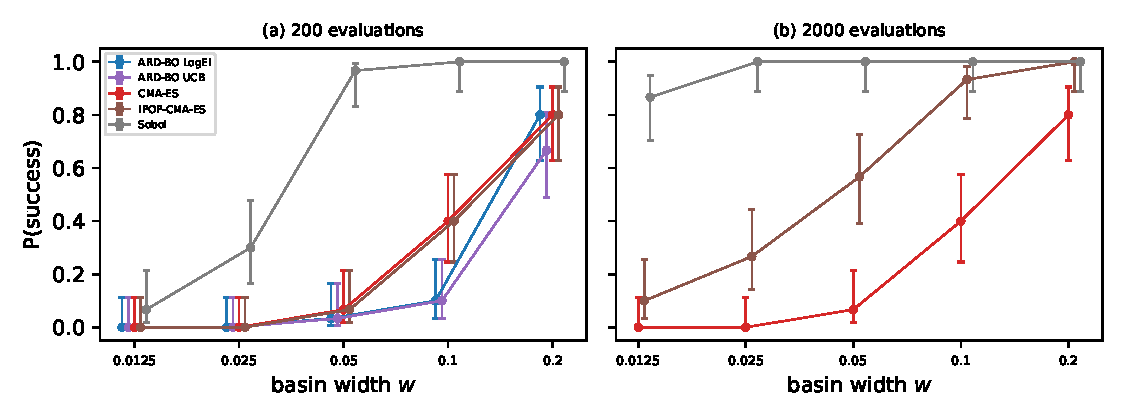
\includegraphics[width=\linewidth]{fig4_e3}\caption{E3, decoy-basin function in $d=2$:
probability that the best point lies in the narrow global basin against its width $w$, 95\% Wilson intervals, 30 seeds,
at 200 (a) and 2000 evaluations (b; CMA-ES, IPOP, Sobol).}\label{fig:e3}\end{figure}
\begin{table*}[t]\centering\resizebox{\textwidth}{!}{\begin{tabular}{rcccccc}
\toprule
$n$ & $w$ & LogEI-BO & UCB-BO & CMA-ES & IPOP & Sobol \\
\midrule
200 & 0.2 & 0.80 & 0.67 & 0.80 & 0.80 & 1.00 \\
200 & 0.1 & 0.10 & 0.10 & 0.40 & 0.40 & 1.00 \\
200 & 0.05 & 0.03 & 0.03 & 0.07 & 0.07 & 0.97 \\
200 & 0.025 & 0.00 & 0.00 & 0.00 & 0.00 & 0.30 \\
200 & 0.0125 & 0.00 & 0.00 & 0.00 & 0.00 & 0.07 \\
2000 & 0.2 & -- & -- & 0.80 & 1.00 & 1.00 \\
2000 & 0.1 & -- & -- & 0.40 & 0.93 & 1.00 \\
2000 & 0.05 & -- & -- & 0.07 & 0.57 & 1.00 \\
2000 & 0.025 & -- & -- & 0.00 & 0.27 & 1.00 \\
2000 & 0.0125 & -- & -- & 0.00 & 0.10 & 0.87 \\
\bottomrule
\end{tabular}
}\caption{E3 success probabilities: fraction
of 30 seeds whose best point lies in the narrow global basin of the decoy-basin function ($d=2$), by budget $n$ and width
$w$. BO is not run at 2000 evaluations.}\label{tab:e3}\end{table*}

\paragraph{Question and setup.}
Does a narrow global basin next to a broad decoy defeat the methods, and do exploration (UCB) and restarts (IPOP) help?
The design is in Table~\ref{tab:design}.

\paragraph{Result.}
Success falls with width for every method (Figure~\ref{fig:e3}, Table~\ref{tab:e3}). At 200 evaluations LogEI-BO succeeds
on $\numeprobtwohundredwidelogei$ of seeds at the widest basin and $\numeprobtwohundrednarrowlogei$ at the narrowest, UCB-BO
on $\numeprobtwohundredwideucb$ and $\numeprobtwohundrednarrowucb$, CMA-ES on $\numeprobtwohundredwidecma$ and
$\numeprobtwohundrednarrowcma$. UCB does not beat LogEI on the narrowest basin ($\numethreeucbminuslogeinarrow$; both fail on
every seed), so this part of H3 is not resolved, and on the widest basin LogEI is better ($\numethreeucbminuslogeiwide$).
IPOP beats default CMA-ES at 2000 evaluations, pooled over widths $\numethreeipoppooled$, reaching
$\numeprobtwothousandnarrowipop$ at the narrowest basin where CMA-ES stays at $\numeprobtwothousandnarrowcma$. Unexpectedly,
Sobol is best: $\numeprobtwohundredwidesobol$ and $\numeprobtwohundrednarrowsobol$ at 200 evaluations and
$\numeprobtwothousandnarrowsobol$ at the narrowest basin with 2000 points.

\paragraph{Interpretation.}
H3 is partly supported: two parts hold and one is not resolved.
% CHECK: based on results/summary/e3_sanity.csv and e3_exploration_check.txt (no macros).
A sanity check rules out an implementation error: after the initial design almost all BO evaluations sit at the bottom
of the broad basin, BO's few narrow-width successes come from its initial points, and UCB with a much larger weight
becomes space filling and succeeds more often. A smooth GP fitted in the bowl has no reason to predict a narrow dip.

\paragraph{Caveat.}
Only $d=2$ was run and the UCB weight was not tuned; with $2d=4$ initial points every width is far below the design
spacing, so the registered statement about the initial design cannot be separated from ``narrow basins are hard''.

\section{Follow-up: TuRBO rotation penalty}
% figures: fig5_ablation
% tables: tab_ablation
% macros: ablation*
\begin{figure}[t]\centering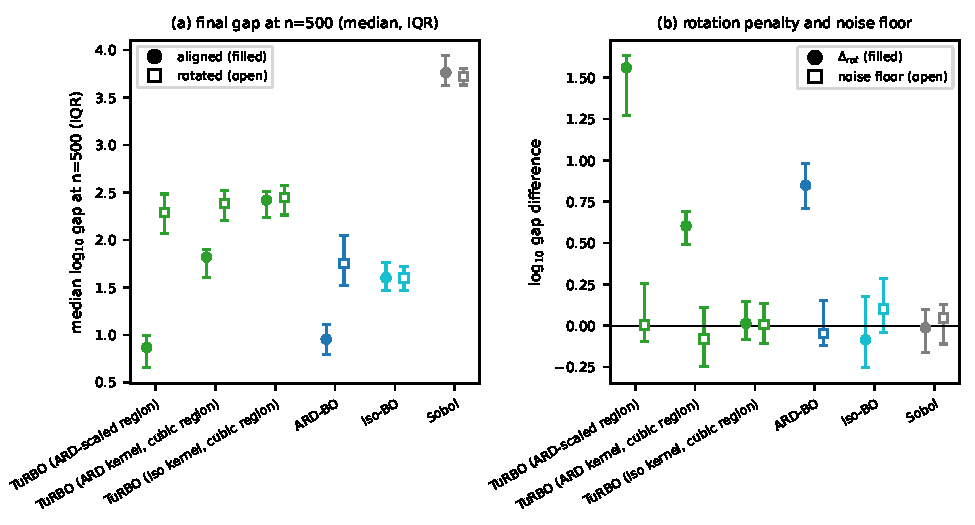
\includegraphics[width=\linewidth]{fig5_ablation}\caption{TuRBO ablation on the E2 primary
instances ($d=10$, $\kappa=10^4$, 500 evaluations, 30 seeds). (a) Median final $\log_{10}$ gap with IQR, aligned (filled)
and rotated (open). (b) $\Drot$ (filled) and aligned-replicate noise floor (open), median with 95\% CI. ARD-BO, iso-BO and
Sobol are the E2 runs.}\label{fig:ablation}\end{figure}
\begin{table*}[t]\centering\resizebox{\textwidth}{!}{\begin{tabular}{lcccc}
\toprule
Method & Aligned & Rotated & $\Delta_{rot}$ [95\% CI] & Noise floor [95\% CI] \\
\midrule
TuRBO (ARD-scaled region) & 0.87 & 2.29 & 1.56 [1.27, 1.63] & 0.00 [-0.09, 0.25] \\
TuRBO (ARD kernel, cubic region) & 1.82 & 2.39 & 0.60 [0.49, 0.69] & -0.08 [-0.24, 0.11] \\
TuRBO (iso kernel, cubic region) & 2.42 & 2.45 & 0.01 [-0.09, 0.15] & 0.01 [-0.11, 0.14] \\
ARD-BO & 0.95 & 1.75 & 0.85 [0.71, 0.98] & -0.05 [-0.12, 0.15] \\
iso-BO & 1.60 & 1.60 & -0.09 [-0.25, 0.18] & 0.10 [-0.04, 0.29] \\
Sobol & 3.76 & 3.72 & -0.01 [-0.16, 0.10] & 0.05 [-0.11, 0.13] \\
\bottomrule
\end{tabular}
}\caption{TuRBO ablation ($d=10$, $\kappa=10^4$, 500 evaluations, 30 paired seeds): median final $\log_{10}$ gap,
$\Drot$ and aligned-replicate noise floor (95\% bootstrap CIs). Default TuRBO scales its trust region by the ARD
lengthscales; the variants use a cubic region.}\label{tab:ablation}\end{table*}

\begin{table*}[t]\centering\resizebox{\textwidth}{!}{\begin{tabular}{llcl}
\toprule
 & Statistic & Estimate [95\% CI] & Outcome (rule in \texttt{predictions.md}) \\
\midrule
H1 & $S=D(10)-D(2)$, ellipsoid $\kappa=100$ & 0.34 [-0.55, 1.14] & $0<S<0.5$: direction only \\
H1 & $S=D(10)-D(2)$, Rosenbrock & 0.65 [0.03, 1.22] & $S\geq0.5$: size supported \\
H1 & $S=D(10)-D(2)$, ellipsoid $\kappa=10^4$ (supplement) & 0.90 [0.44, 1.35] & $S\geq0.5$: size supported \\
H2 & $\Delta_{rot}$ interaction, ARD-BO $-$ iso-BO & 0.89 [0.54, 1.20] & supported (CI excludes 0) \\
H2 & $\Delta_{rot}$ interaction, sep-CMA-ES $-$ CMA-ES & 0.76 [0.62, 0.93] & supported (CI excludes 0) \\
H2 & $\rho$ at $n=200$, aligned ($\rho$ $\geq$ 0.5) & 0.998 [0.997, 0.999] (IQR) & threshold met \\
H2 & $\rho$ at $n=200$, rotated ($\rho$ $\leq$ 0.2) & 0.168 [0.143, 0.182] (IQR) & threshold met \\
H3 & $P(w{=}0.2)-P(w{=}0.0125)$, every method & 0.13 to 0.93 & supported (all CIs exclude 0) \\
H3 & UCB $-$ LogEI success, $w=0.0125$ & 0.00 [0.00, 0.00] & not resolved \\
H3 & IPOP $-$ CMA-ES success, pooled, $n=2000$ & 0.32 [0.25, 0.39] & supported \\
H4 & Spearman($c^*$, budget), ellipsoid & 0.97 & $c^*$ increases with budget \\
H4 & Spearman($c^*$, budget), Rosenbrock & 0.97 & $c^*$ increases with budget \\
H5 & $\hat\alpha$, $d\geq10$, $\tau=10$ & 2.022 [1.988, 2.056] & refuted (CI excludes 1.87) \\
Follow-up & cubic ARD $\Delta_{rot}$ & 0.60 [0.49, 0.69] & prediction met \\
Follow-up & isotropic $\Delta_{rot}$ & 0.01 [-0.09, 0.15] & prediction met \\
\bottomrule
\end{tabular}
}\caption{Pre-registered statistics and outcomes under the rules in \texttt{predictions.md} and the addenda (medians with
95\% bootstrap CIs unless marked IQR; H4: Spearman correlation of median $c^*$ with budget; H1 rows: see the amendment in
Section~1).}\label{tab:predictions}\end{table*}

\paragraph{Question and setup.}
Is TuRBO's excess rotation penalty over ARD-BO caused by its ARD-scaled trust region? Two variants, an ARD kernel with a
cubic region and an isotropic kernel (cubic region), were run on the E2 instances. Registered prediction: for cubic ARD, $\Drot$ in
$[0.45,1.25]$ with a CI excluding 0 and a negative contrast with the default; for isotropic, $|\Drot|\leq0.3$ with a CI
containing 0.

\paragraph{Result.}
Both predictions are met (Table~\ref{tab:ablation}, Figure~\ref{fig:ablation}): cubic ARD $\Drot=\numablationdrotcubic$
against $\numablationdrotdefault$ for the default (contrast $\numablationcontrastcubicdefault$), isotropic
$\numablationdrotiso$, with noise floors $\numablationfloordefault$, $\numablationfloorcubic$ and $\numablationflooriso$.

\paragraph{Interpretation.}
The penalty does not fall through a better rotated result: the rotated median gap barely changes
($\numablationrotateddefault$, $\numablationrotatedcubic$, $\numablationrotatediso$), while the aligned one degrades from
$\numablationaligneddefault$ to $\numablationalignedcubic$ and $\numablationalignediso$. The ARD-scaled region lets TuRBO
exploit alignment; removing it removes the aligned advantage rather than the cost of rotation. Caveat: reference
defaults only, on one problem, dimension and budget.

\section{Predictions and outcomes}
% figures: none
% tables: tab_predictions
% macros: none
% The tab_predictions float is defined at the start of Section 6 so that the two-column float can appear by this page.
Table~\ref{tab:predictions} collects the pre-registered statistics: \textbf{H1} and \textbf{H3} are partly supported,
\textbf{H2} and \textbf{H4} are supported, \textbf{H5} is not supported, and the \textbf{follow-up} predictions are met
for a different reason than intended.

\section{Discussion and limitations}
% figures: none
% tables: none
% macros: none
\paragraph{What survives.}
The central claim, that BO's advantage depends on problem--method fit rather than general superiority, holds within the
tested range: ARD-BO and TuRBO gain most where the problem matches their axis-aligned modelling;
BO's lead is largest early and at low dimension; its overhead pays off only for expensive evaluations, with a break-even
cost rising steeply with dimension and budget; and on a deceptive multimodal function no method beat Sobol sampling.
This qualifies the finding that BO is preferable at limited budgets \citep{santoni2024hdbo}.

\paragraph{Limitations.}
All functions are synthetic and smooth. CPU time (one BO run at $d=10$ with 1000 evaluations took hours) limited E1 to
$d\leq10$ instead of the planned $d=20$ and E3 to $d=2$; E2 was not run at $\kappa=1$ or 100. Methods use defaults;
the sensitivity grids covered two pilot problems with ten seeds, and TuRBO and the UCB weight were not tuned. Box bounds
break CMA-ES's rotation invariance (E0) by a mechanism not isolated here. The refit check used 10 to 15 seeds, the E3
exploration check six. Overheads come from one CPU under parallel load; noise was not studied. Next tests: E1 at
$d=20$, CMA-ES with other bound handling, and BO with a full-metric kernel on rotated problems.

\bibliographystyle{alpha}
\bibliography{references}

\appendix
\section{Appendix}
\label{sec:appendix}
% sensitivity grids: results/summary/sensitivity_cmaes.csv, sensitivity_bo.csv (table not generated yet)
% refit schedule (A4): results/summary/a4_refit_check.csv, a4_d10_check.csv (table not generated yet)
% correctness anchor: results/summary/anchor.csv (table not generated yet)
% E0 rotation audit: results/summary/e0_rotation.csv (table not generated yet)
% CMA-ES long runs: results/summary/e2_cma_long_reach.csv (table not generated yet)
% H5 other tau: tab_h5 (already in the E1 section)
% E3 sanity checks: results/summary/e3_sanity.csv, e3_exploration_check.txt (table not generated yet)
% macros: none
% CHECK: the appendix summarises CSV files that have no macros; numbers are omitted for that reason.
\paragraph{Correctness anchor.}
The CMA-ES wrapper evaluates exactly the same points as pycma's reference interface on a bounded test problem, and BO and
TuRBO meet a median-gap threshold on the Branin function that was fixed in advance (\texttt{results/summary/anchor.csv}).

\paragraph{E0: rotation invariance of CMA-ES.}
On the ellipsoid at $d=10$, CMA-ES's rotation penalty is consistent with zero without bounds and positive, with a CI
excluding 0, with the unit box (\texttt{results/summary/e0\_rotation.csv}). A first version of this audit drew instance
and method random numbers from the same stream; its noise floor was non-zero, which exposed the problem. All reported runs
use independent streams.

\paragraph{Sensitivity grids.}
A smaller $\sigma_0$ improved CMA-ES on the rotated-ellipsoid pilot but not on Rosenbrock, a doubled population was worse
in every comparison, and no BO alternative was better on either problem; under the pre-set rule all defaults were kept
(\texttt{results/summary/sensitivity\_*.csv}).
% CHECK: sigma0 = 0.15 secondary interaction from results/summary/e2_primary.csv (no macro).
The $\sigma_0=0.15$ variant, run as a declared secondary variant in E2, keeps the sep-CMA-ES interaction positive with a CI
excluding 0.

\paragraph{GP refit schedule (A4).}
Warm-started refits reached the same marginal likelihood as cold refits with different lengthscales and gave worse BO
results on the rotated ellipsoid. Refitting every ten instead of every five iterations after $n=100$ made no detectable
difference at $d=5$ and $d=10$ under a rule fixed before the runs (\texttt{results/summary/a4\_refit\_check.csv},
\texttt{a4\_d10\_check.csv}).

\end{document}
